Noise in the photodetector or the detector electronics can result in spurious photon signals. 
Most of the time, such spurious signal is filtered out by multiple layers of protection, starting from the so-called ``spike killer'' algorithm at the Level 1 trigger~\cite{CMS_AN_2010-357}. 
Nevertheless, in rare cases, noise in a single ECAL channel coincides with pileup or other energy deposit in the nearby crystals and appear as a high-energy photon cluster.

\begin{figure}[tbp]
  \centering
  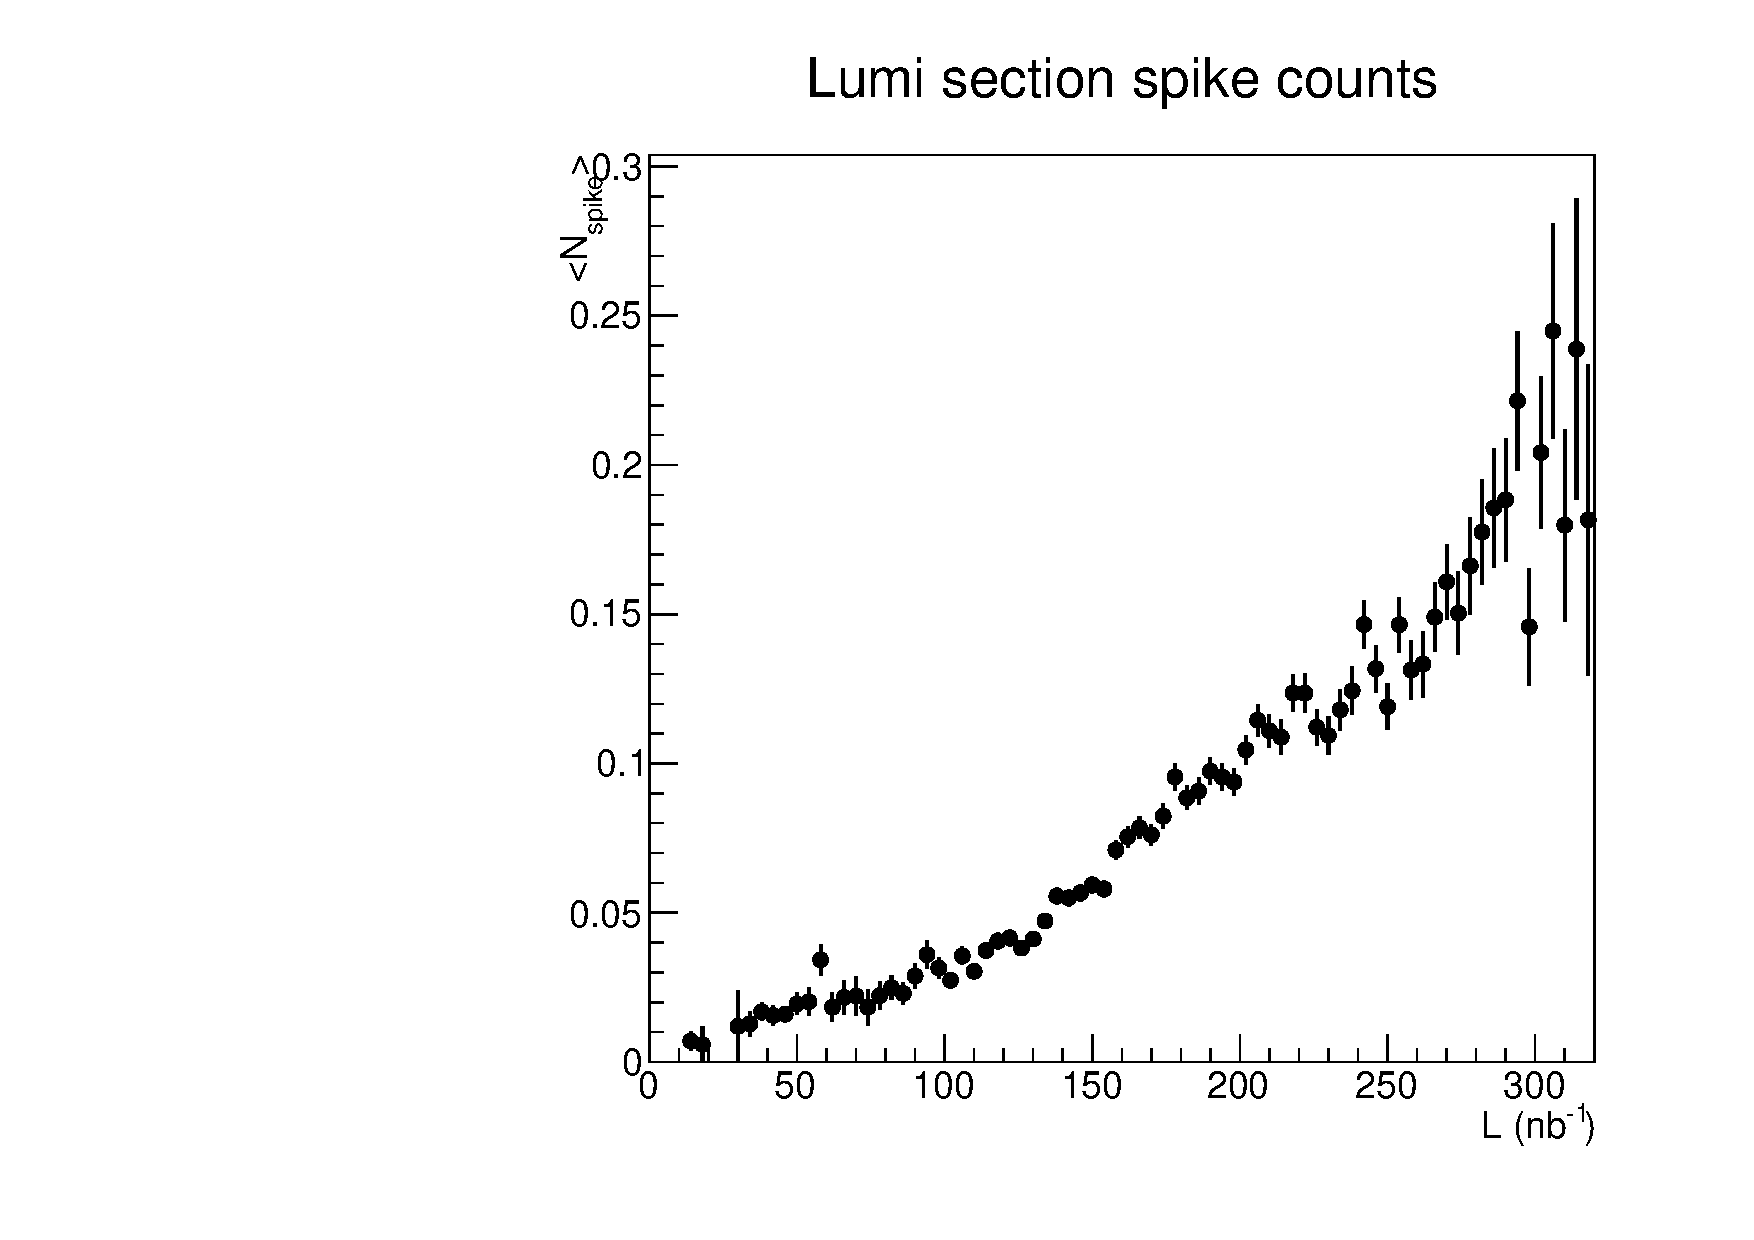
\includegraphics[width=0.45\textwidth]{Reconstruction/Figures/spikes/spike_lumi_scaling.pdf}
  \caption{
    Average number of spike clusters in a luminosity section, identified by $\sieie < 0.001$ and $E > 50\GeV$, in muon-triggered events, versus integrated luminosity of the luminosity section.
  }
  \label{fig:spike_lumi_scaling}
\end{figure}

The origin of ECAL spikes is believed to be interactions of neutrons and other hadronic particles (collectively called neutral hadrons hereafter) with the photocathode material of the ECAL avalanche photo diodes (APD)~\cite{Spike2012}. 
Nuclear fission at the APD surface then causes a large electron avalanche, which is mistaken as a large photon yield scintillation in the ECAL crystal. 
Evidences supporting this hypothesis is documented in Reference~\cite{CMS_AN_2010-357}. 
In Figure~\ref{fig:spike_lumi_scaling}, scaling of the rate of spikes with the instantaneous luminosity is confirmed, up to much higher luminosity values than was observed at the time when Reference~\cite{CMS_AN_2010-357} was written.

A known feature of such spurious photon clusters is that the recorded pulse shape of the seed crystal, \ie, the channel with the noise, is not what is expected from a real electromagnetic shower in ECAL. 
In particular, this translates to a distinctive early rec hit time distribution, since the rec hit time is extracted from a fit to the pulse shape assuming a normal pulse.

In the normal CMS data reconstruction, rec hits that are tagged as spike-like are ignored in clustering. 
Rec hits are tagged as spikes if there is very little energy deposit recorded in the surrounding crystals, or if the reconstructed time is out of an allowed window.
Identical algorithms are employed in the HLT and offline reconstructions.

\begin{figure}[htbp]
  \centering
  \resizebox{\textwidth}{!}{
    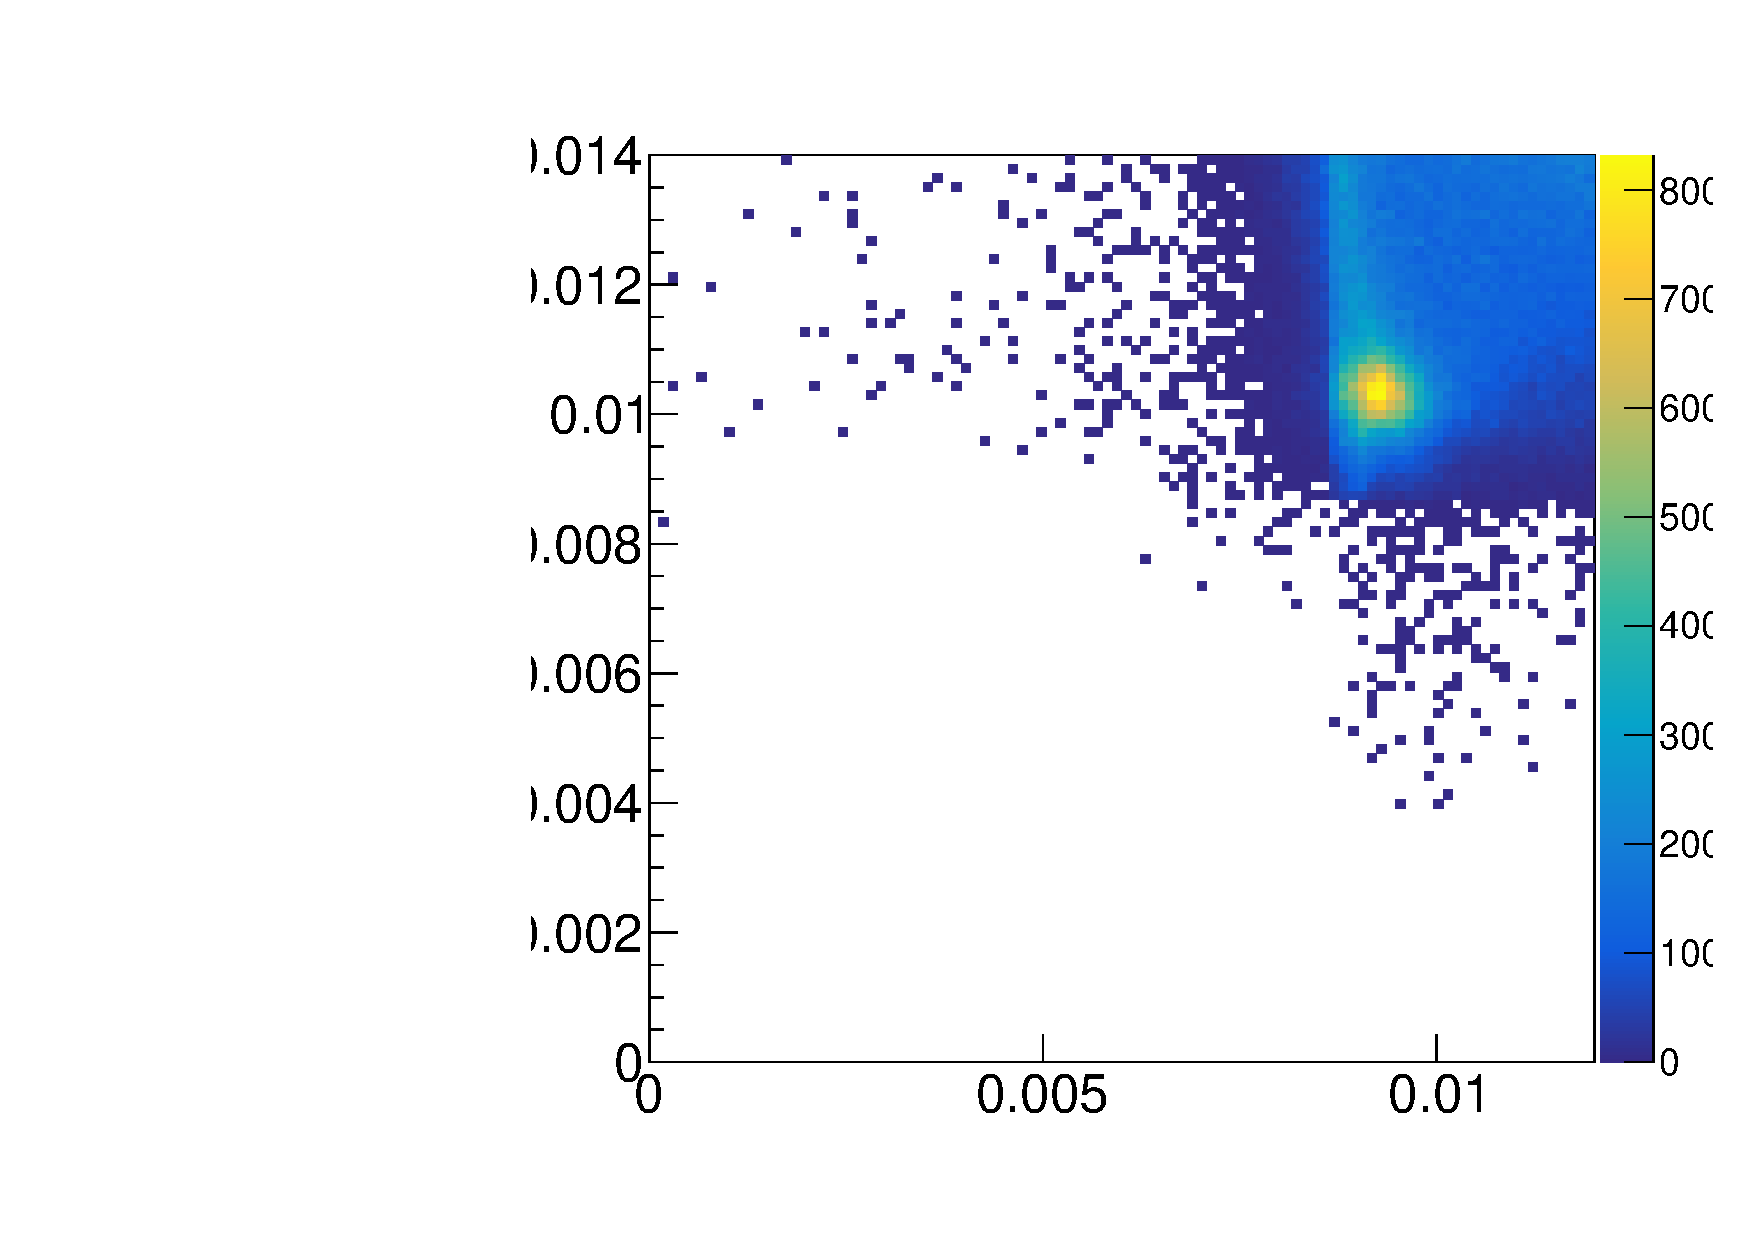
\includegraphics[]{Reconstruction/Figures/spikes/showershapes_standard.pdf}
    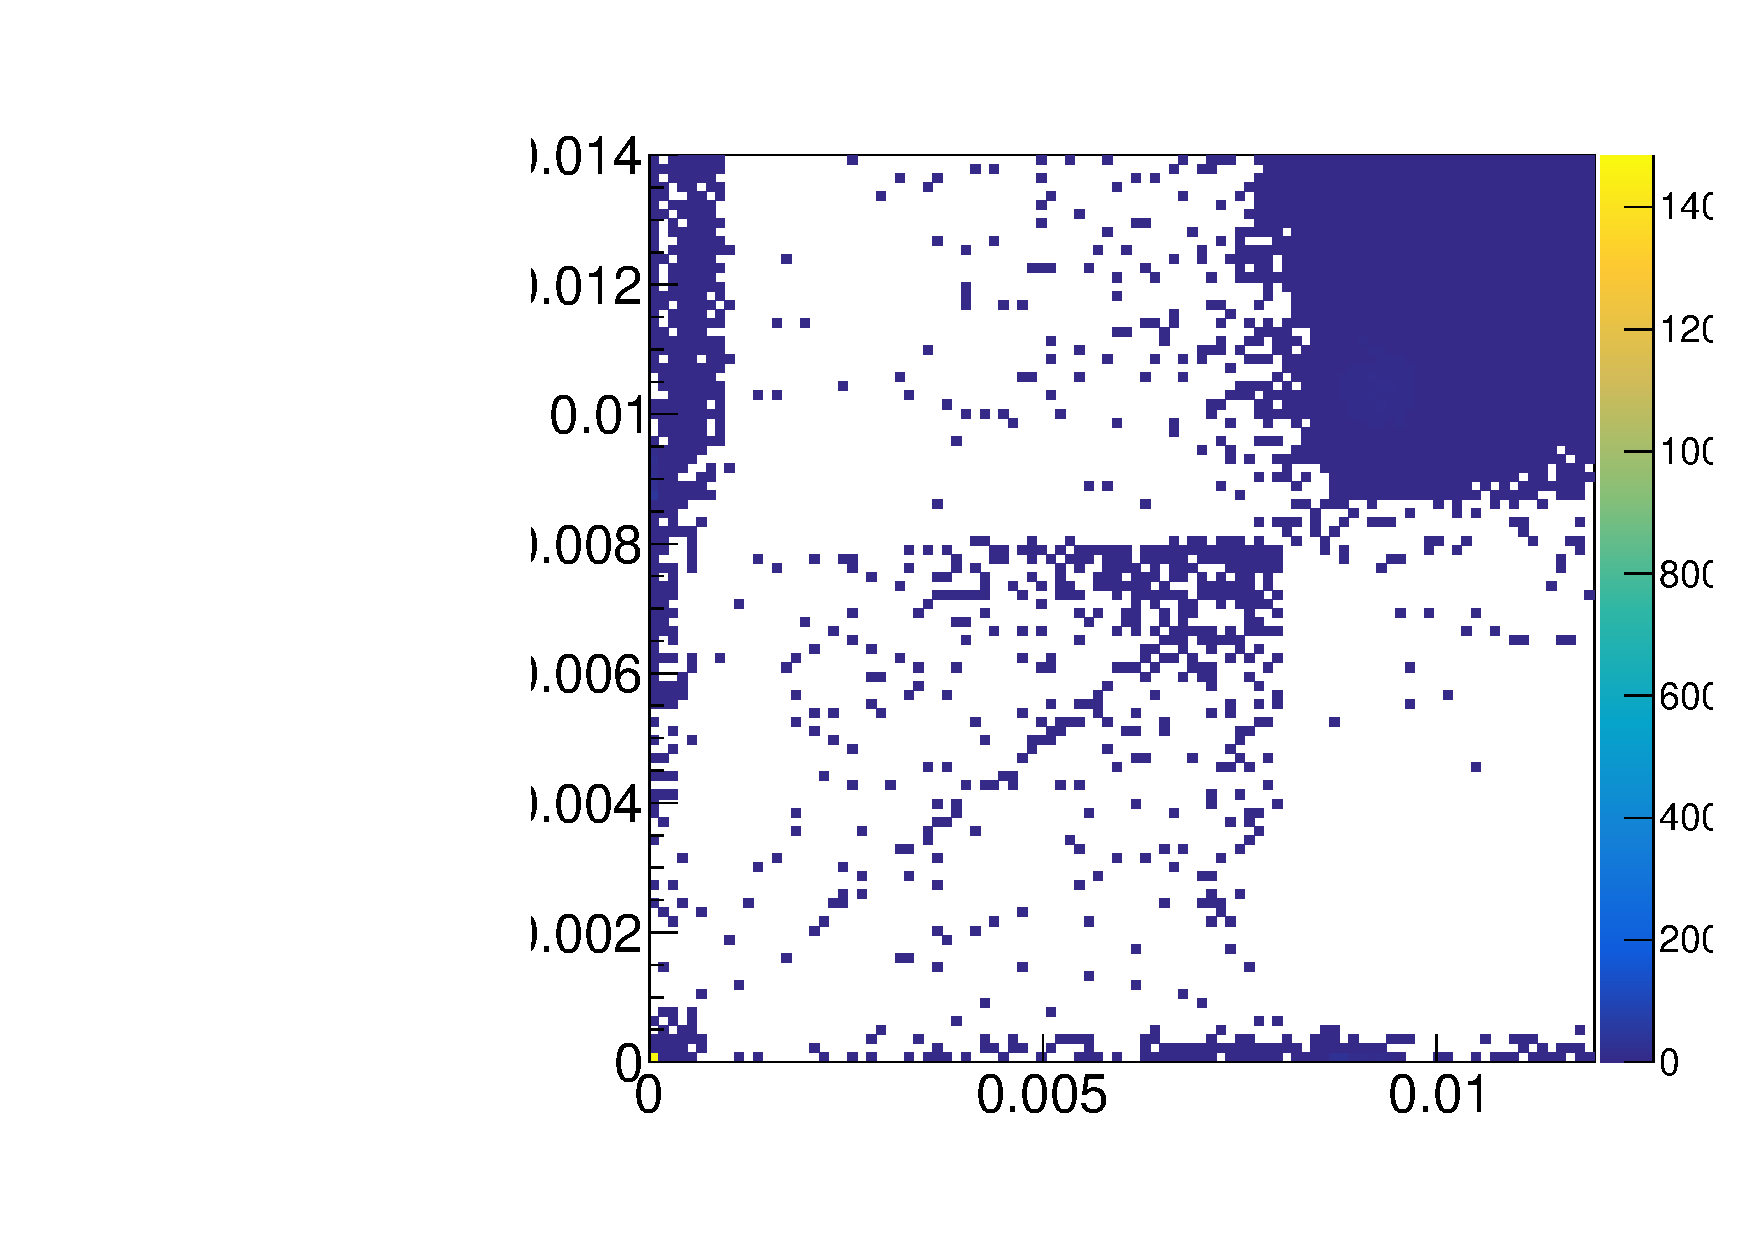
\includegraphics[]{Reconstruction/Figures/spikes/showershapes_uncleaned.pdf}
  }
  \caption{
    Two-dimensional distributions in \sipip\ and \sieie\ of ECAL clusters in the standard reconstruction (left) and the special reconstruction with no spike cleaning (right).
  }
  \label{fig:showershape_map}
\end{figure}

To study an unbiased spike sample, ECAL DIGI samples stored in the SingleMuon AOD datasets are reconstructed into ECAL clusters with no spike cleaning applied. 
DIGIs associated with the standard and ``uncleaned'' photon objects are stored in AOD, and ones for the uncleaned photons is rich in spike-like hits. 
Figure~\ref{fig:showershape_map} shows how narrow clusters are cleaned away in the normal reconstruction.

\begin{figure}[htbp]
  \centering
  \resizebox{\textwidth}{!}{
    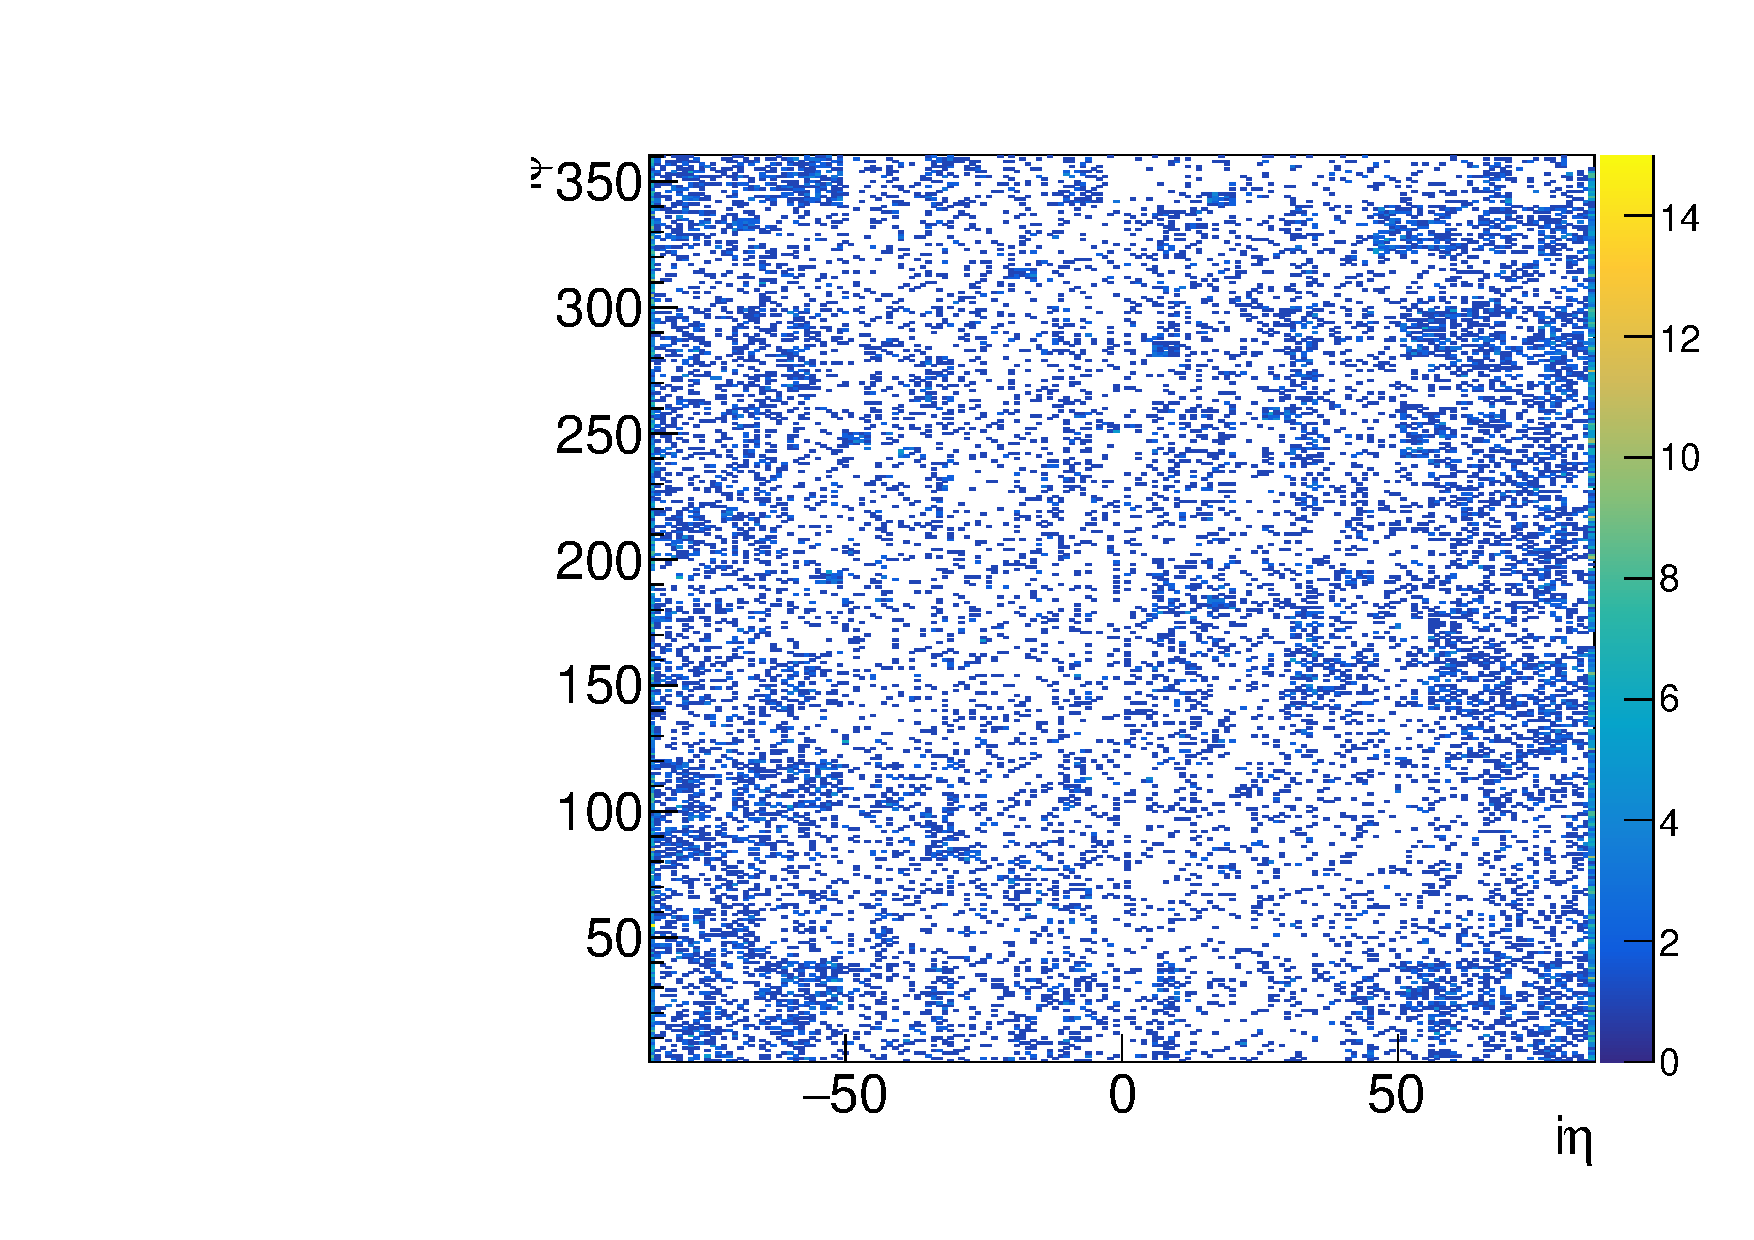
\includegraphics[]{Reconstruction/Figures/spikes/spike_map.pdf}
    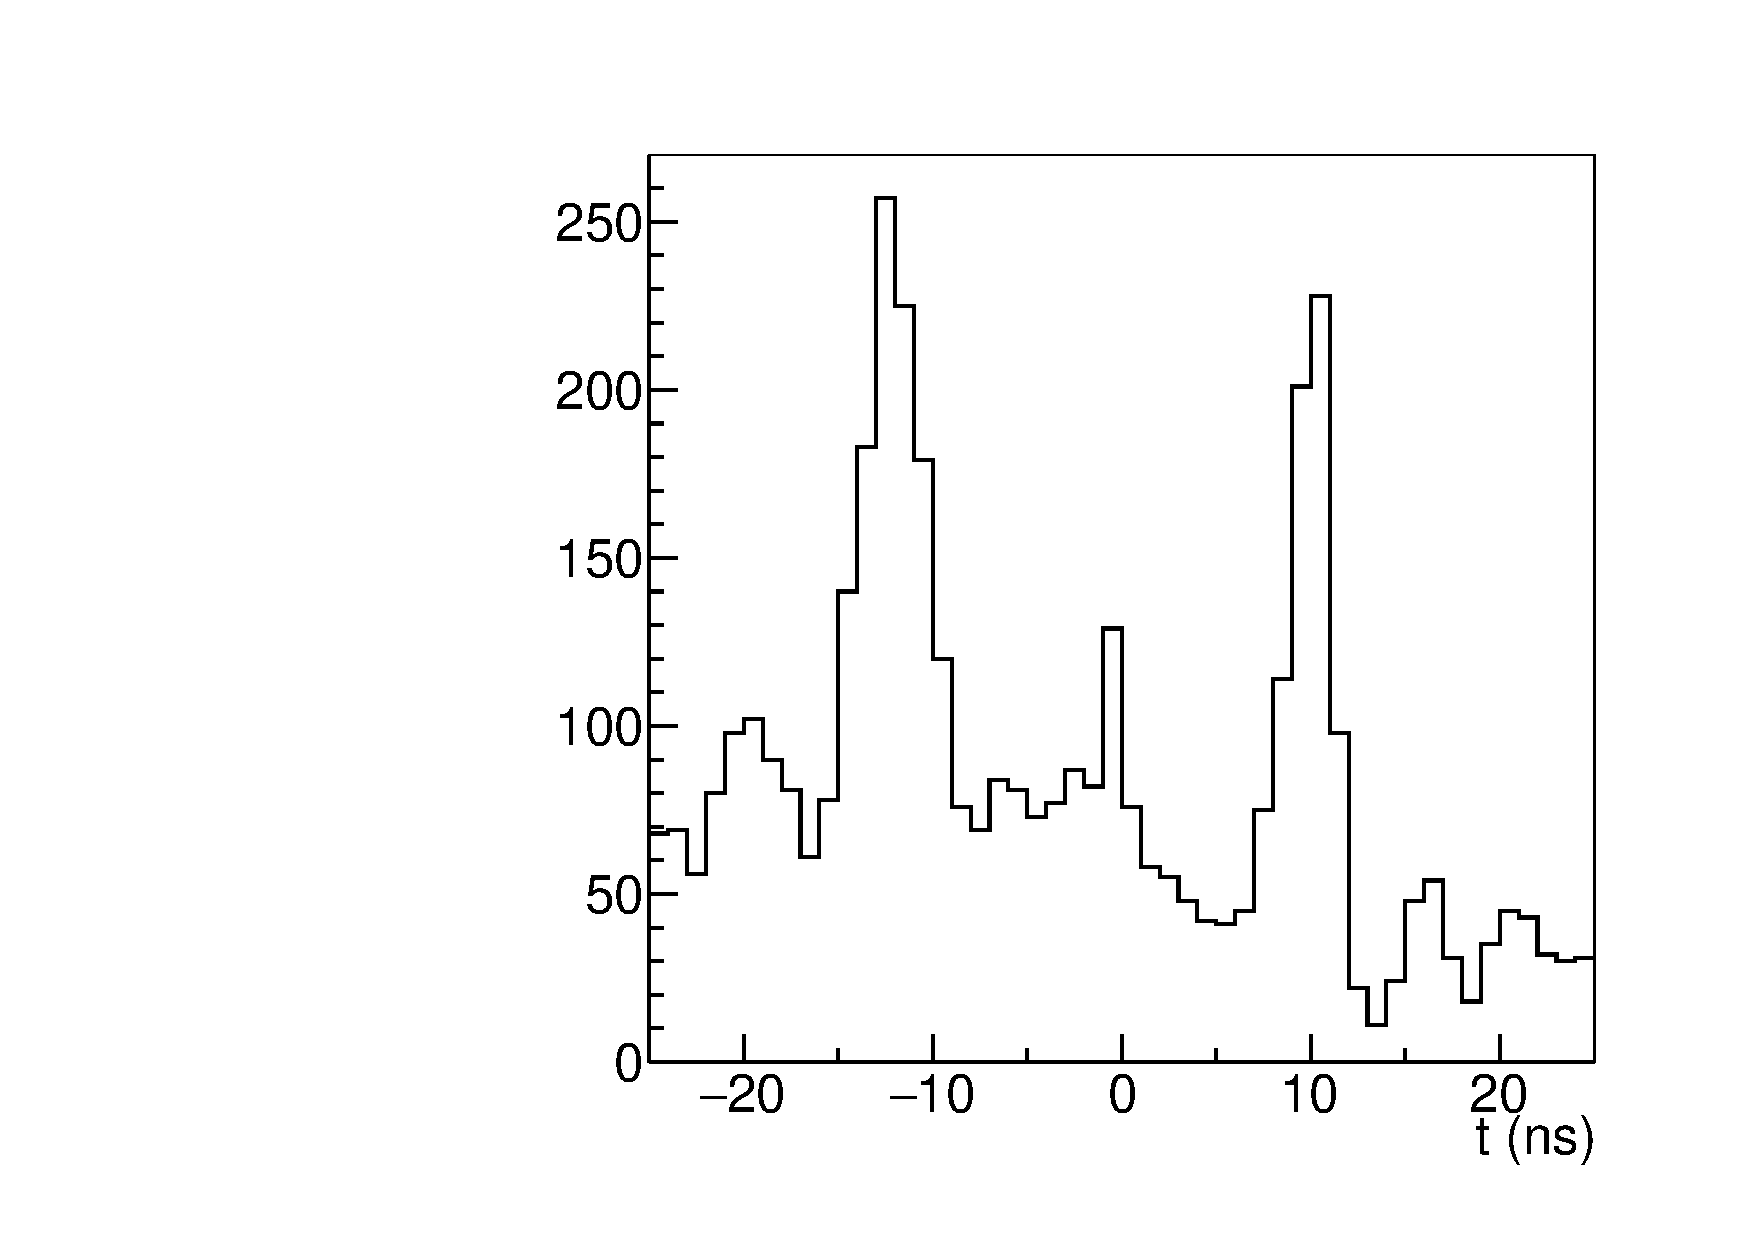
\includegraphics[]{Reconstruction/Figures/spikes/spike_time.pdf}
  }
  \caption{
    $\eta$--$\phi$ and time distributions of seed hits of narrow ($\sieie < 0.001$) clusters.
  }
  \label{fig:spike_distributions}
\end{figure}

Figure~\ref{fig:spike_distributions} shows the spacial and temporal distributions of the rec hits seeding narrow ($\sieie < 0.001$) clusters. 
The spacial distribution appears mostly random, indicating that there is no single source of spike-like rec hits. 
The two highest peaks in the time distribution at $t \sim -15\ns$ and $t \sim 10\ns$ are characteristic of pulse shapes, which rise faster than the pulse from the normal scintillation. 
The second peak is understood to come from the next bunch crossing.

\begin{figure}[htbp]
  \centering
  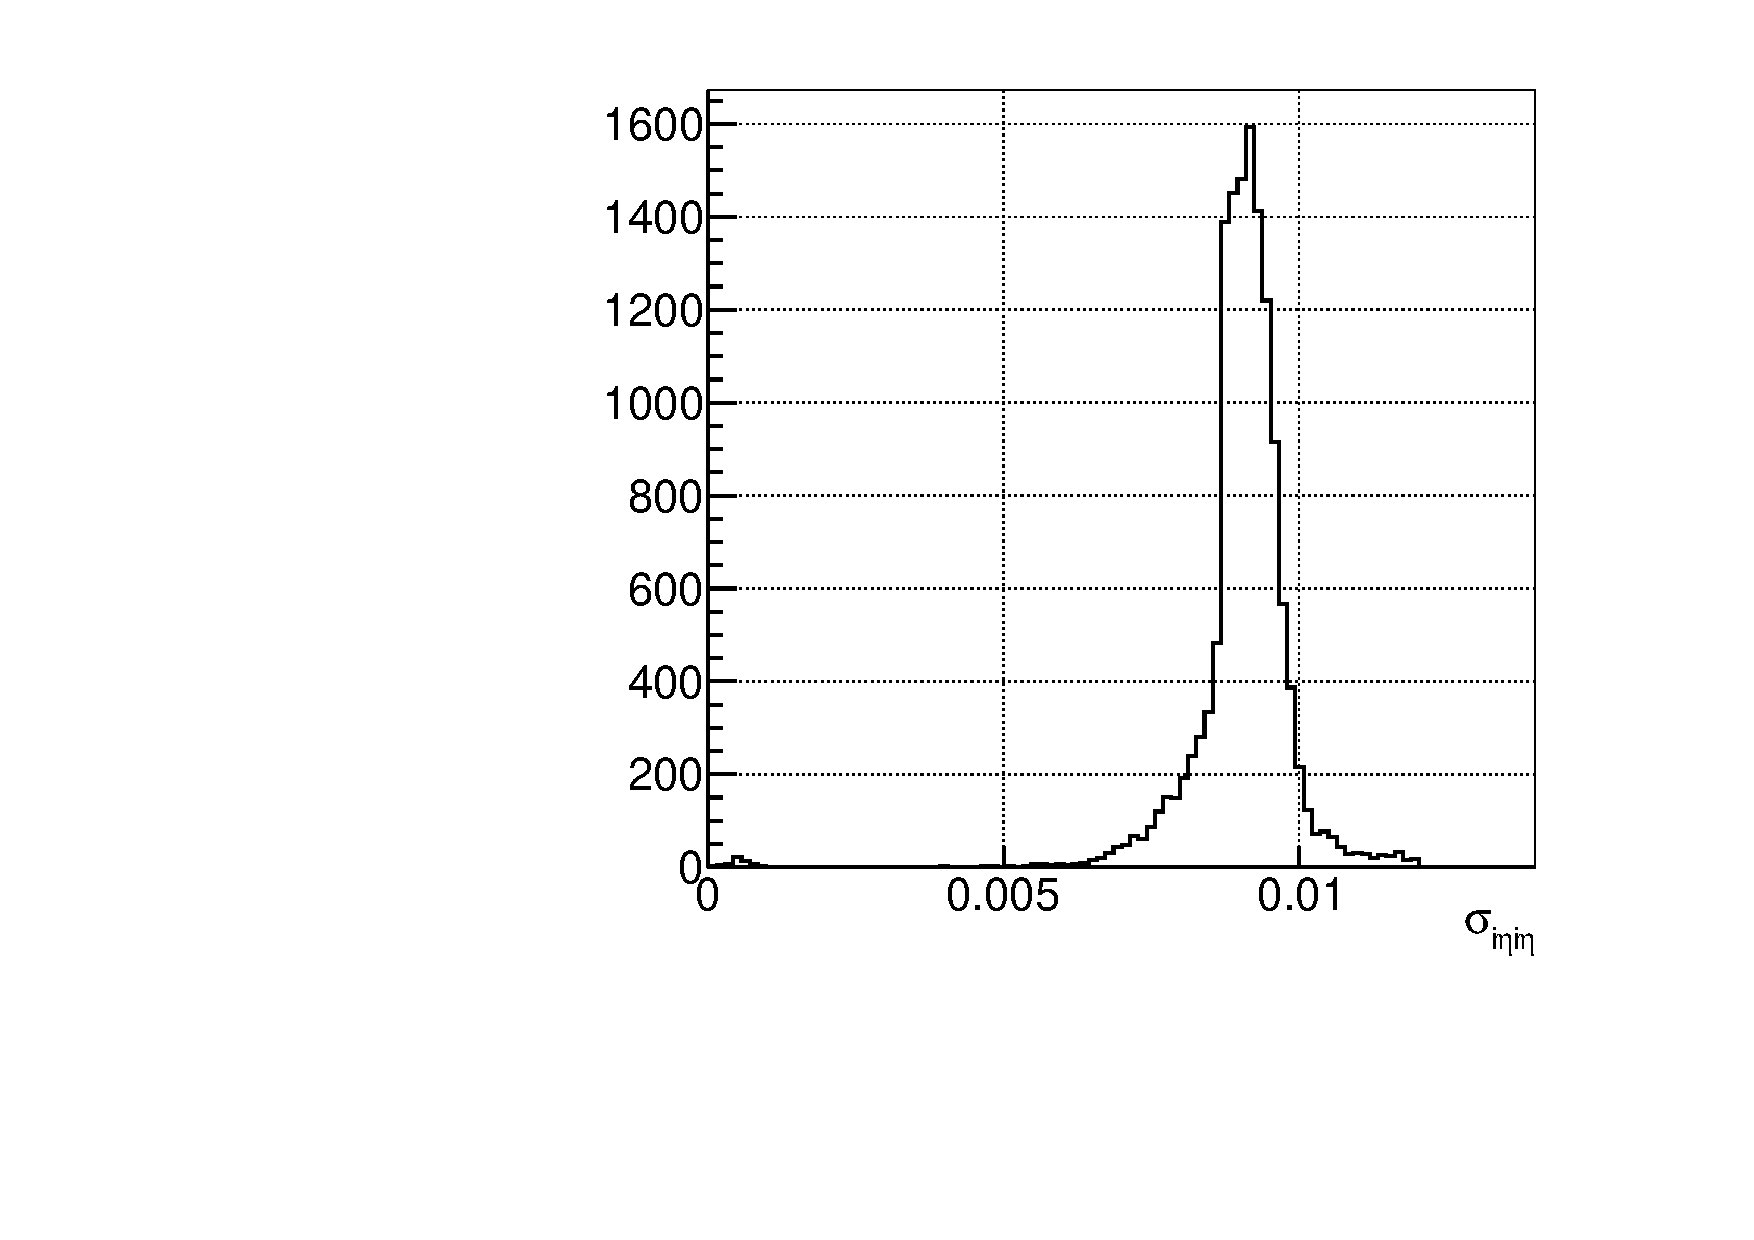
\includegraphics[width=0.45\textwidth]{Reconstruction/Figures/spikes/sieie_mc.pdf}
  \caption{
    \sieie distribution of uncleaned clusters from \gj\ MC simulation.
  }
  \label{fig:sieie_mc}
\end{figure}

The small peak at $t\sim 0$ in the time distribution of Fig.~\ref{fig:spike_distributions} is due to actual ``physical'' clusters that happened to have a very narrow cluster shape. 
By processing the \gj\ MC simulation events through this special reconstruction, we see that about 0.5\% of ECAL clusters from prompt photons have $\sieie < 0.001$ as shown in Figure~\ref{fig:sieie_mc}.

\begin{figure}[htbp]
  \centering
  \resizebox{\textwidth}{!}{
    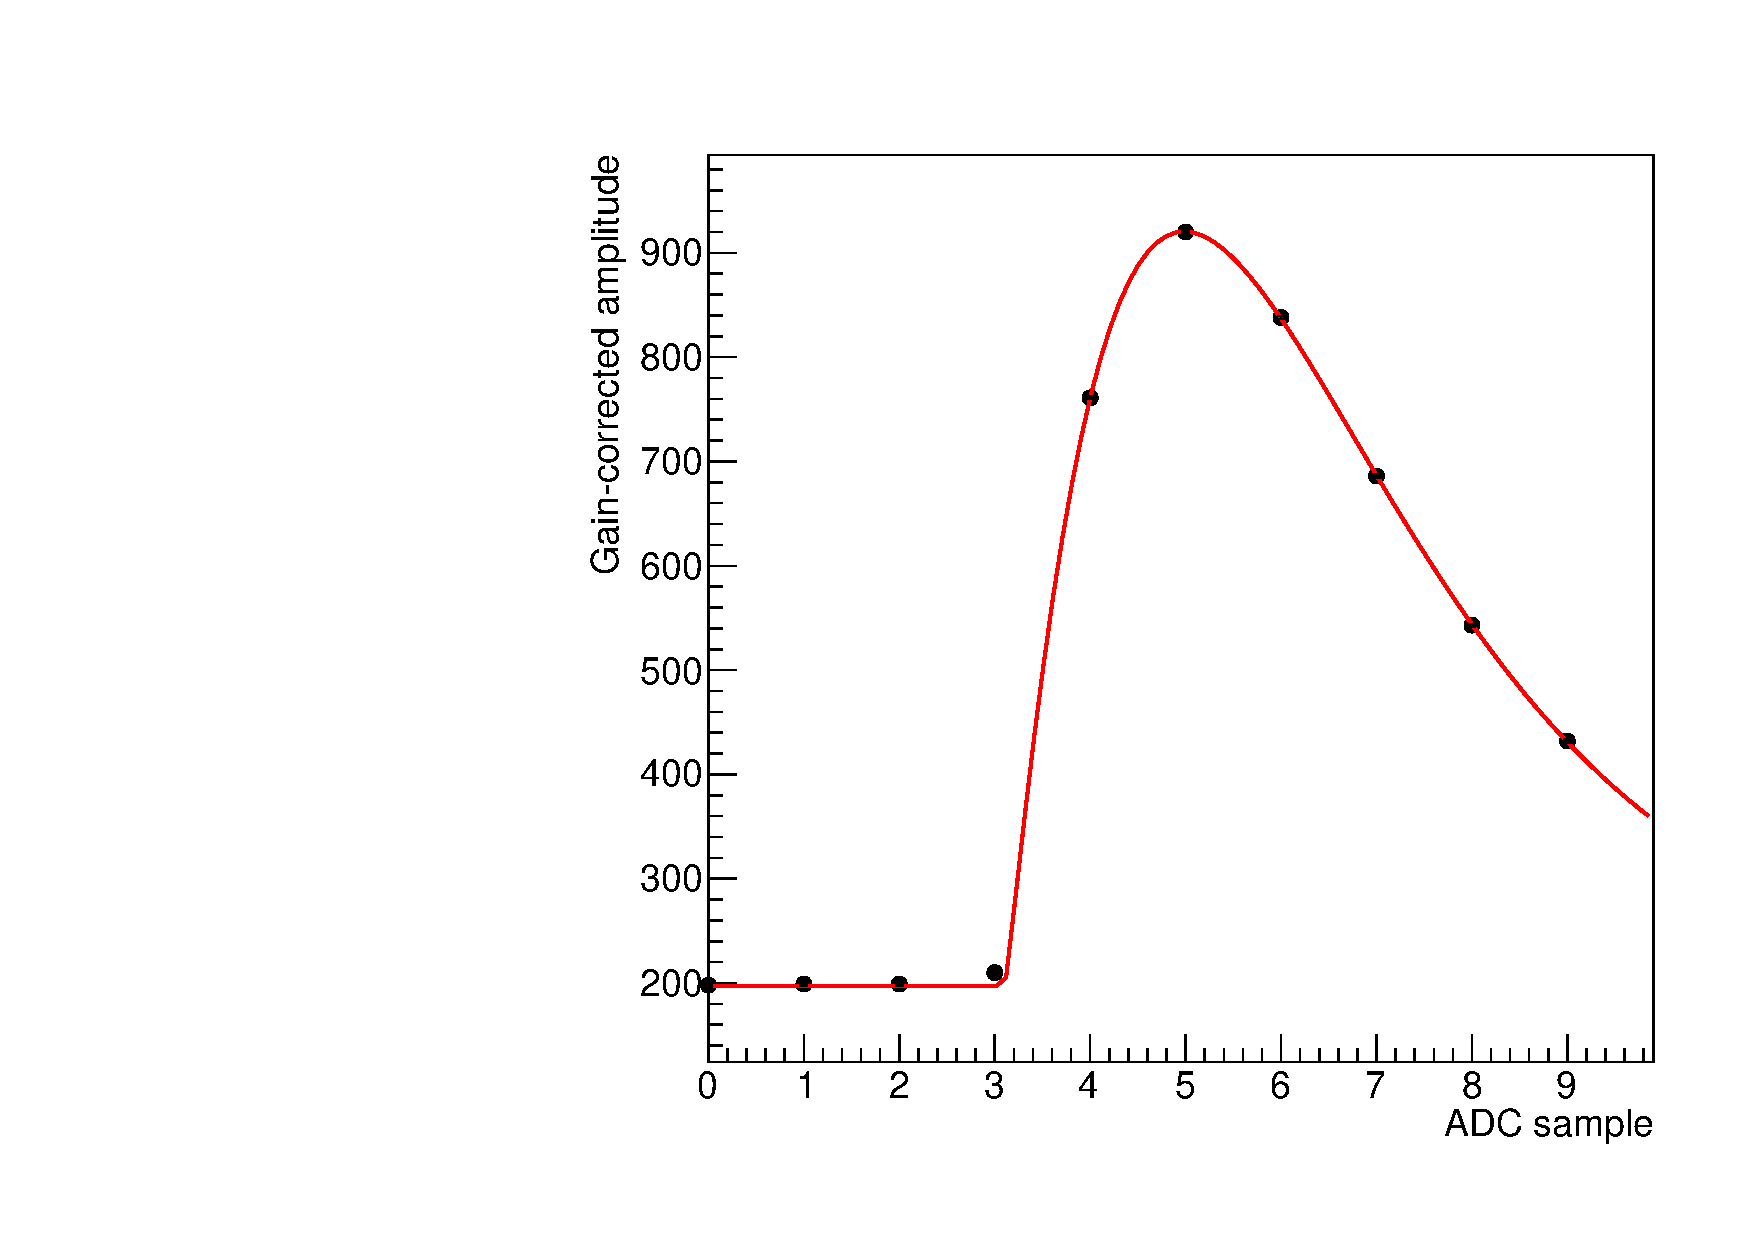
\includegraphics[]{Reconstruction/Figures/spikes/pulse_example_normal.pdf}
    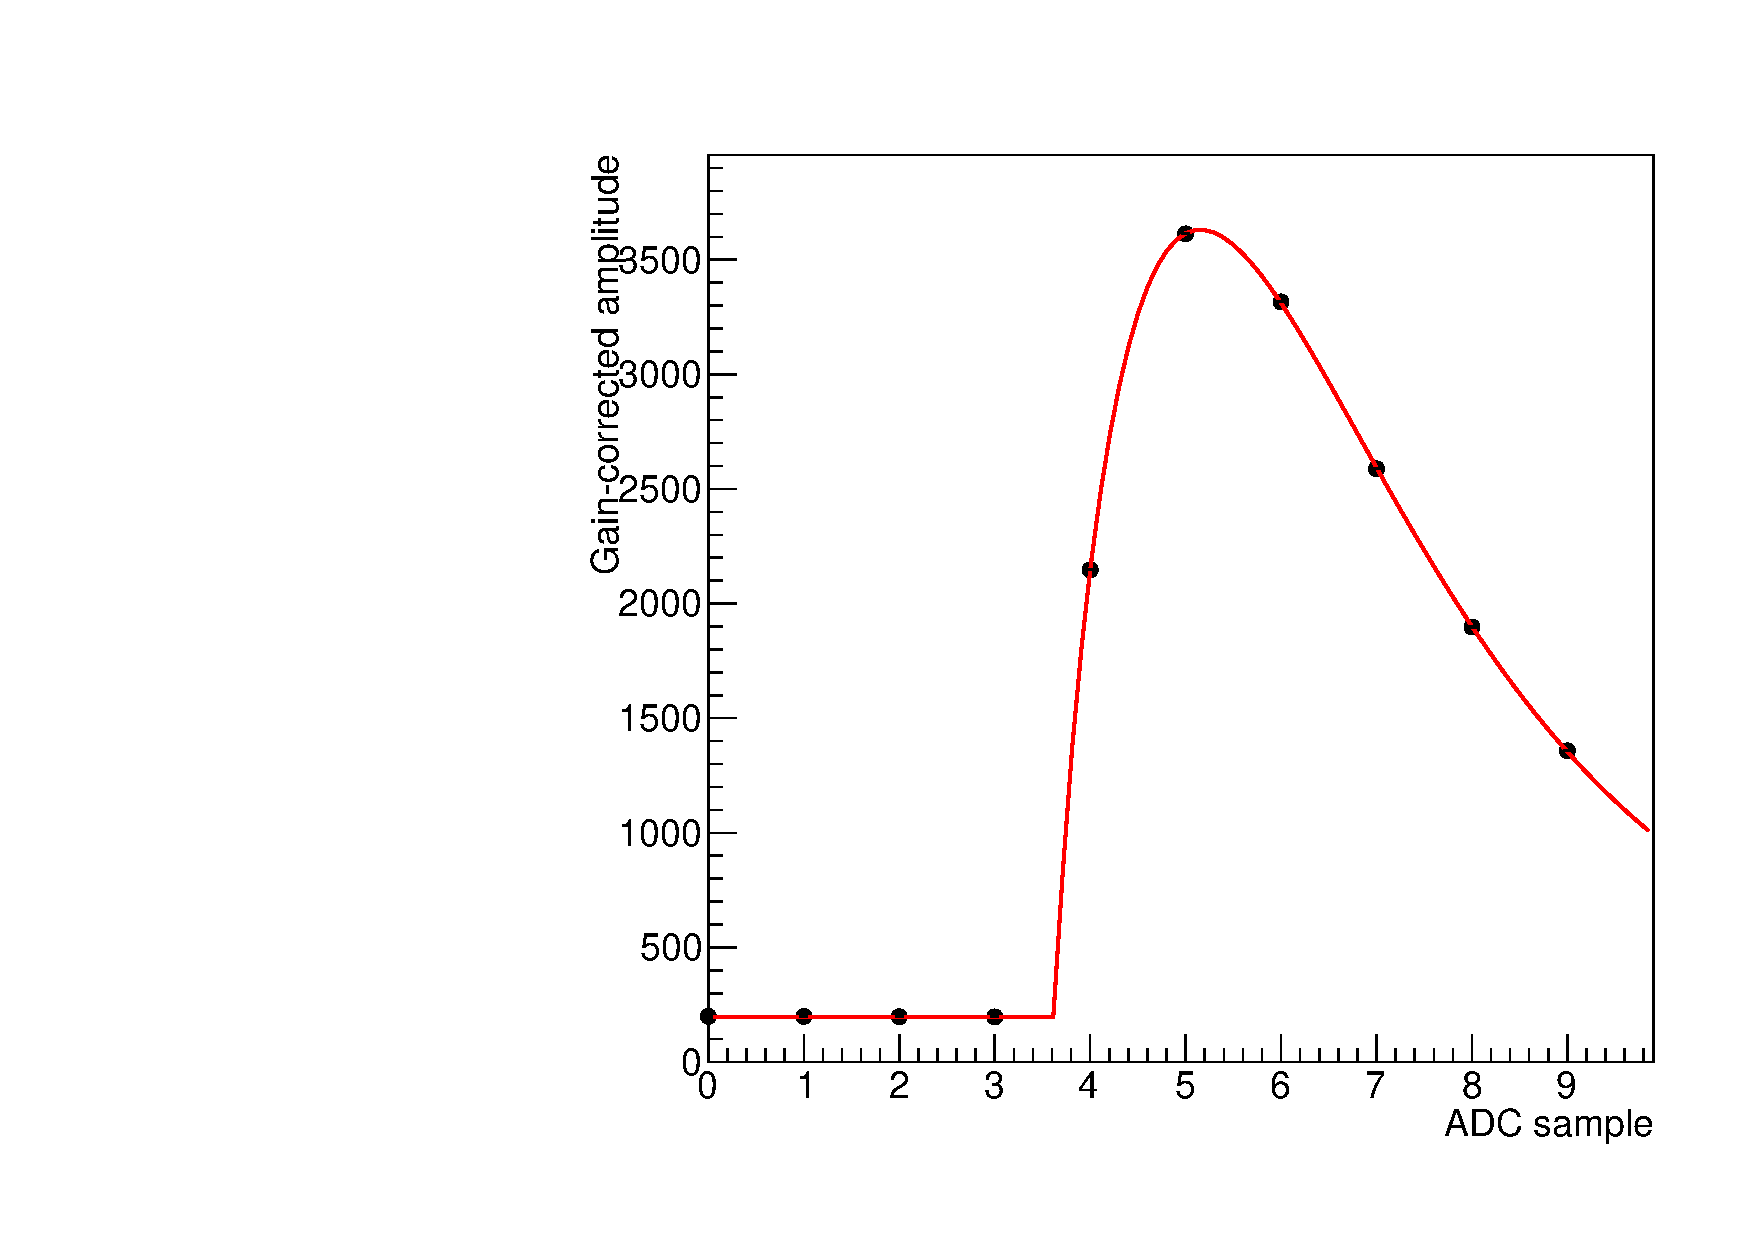
\includegraphics[]{Reconstruction/Figures/spikes/pulse_example_spike.pdf}
  }
  \caption{
    Example ECAL DIGIs and corresponding pulse shapes reconstructed through $\chi^{2}$ fits of Equation~\ref{eqn:pulse_shape}, for normal (left) and spike-like (right) hits.
  }
  \label{fig:pulse_examples}
\end{figure}

To understand the time distribution, one can investigate the original DIGI samples from which rec hits are made. 
At each event readout, a single ECAL channel outputs 10 ADC signals corresponding to a sampling of the analog pulse output of multi-gain preamplifier (MGPA) in range $t_{0} - 125\ns < t < t_{0} + 100\ns$, where $t_{0}$ is the time of the triggering bunch crossing. 
These 10 signal points can be described well by the formula

\begin{equation}
  \label{eqn:pulse_shape}
  f(t) = A \left(1 - \frac{t - \tau}{\alpha\beta}\right)^{\alpha} \exp \left(-\frac{t-\tau}{\beta}\right).
\end{equation}

\begin{figure}[htbp]
  \centering
  \resizebox{\textwidth}{!}{
    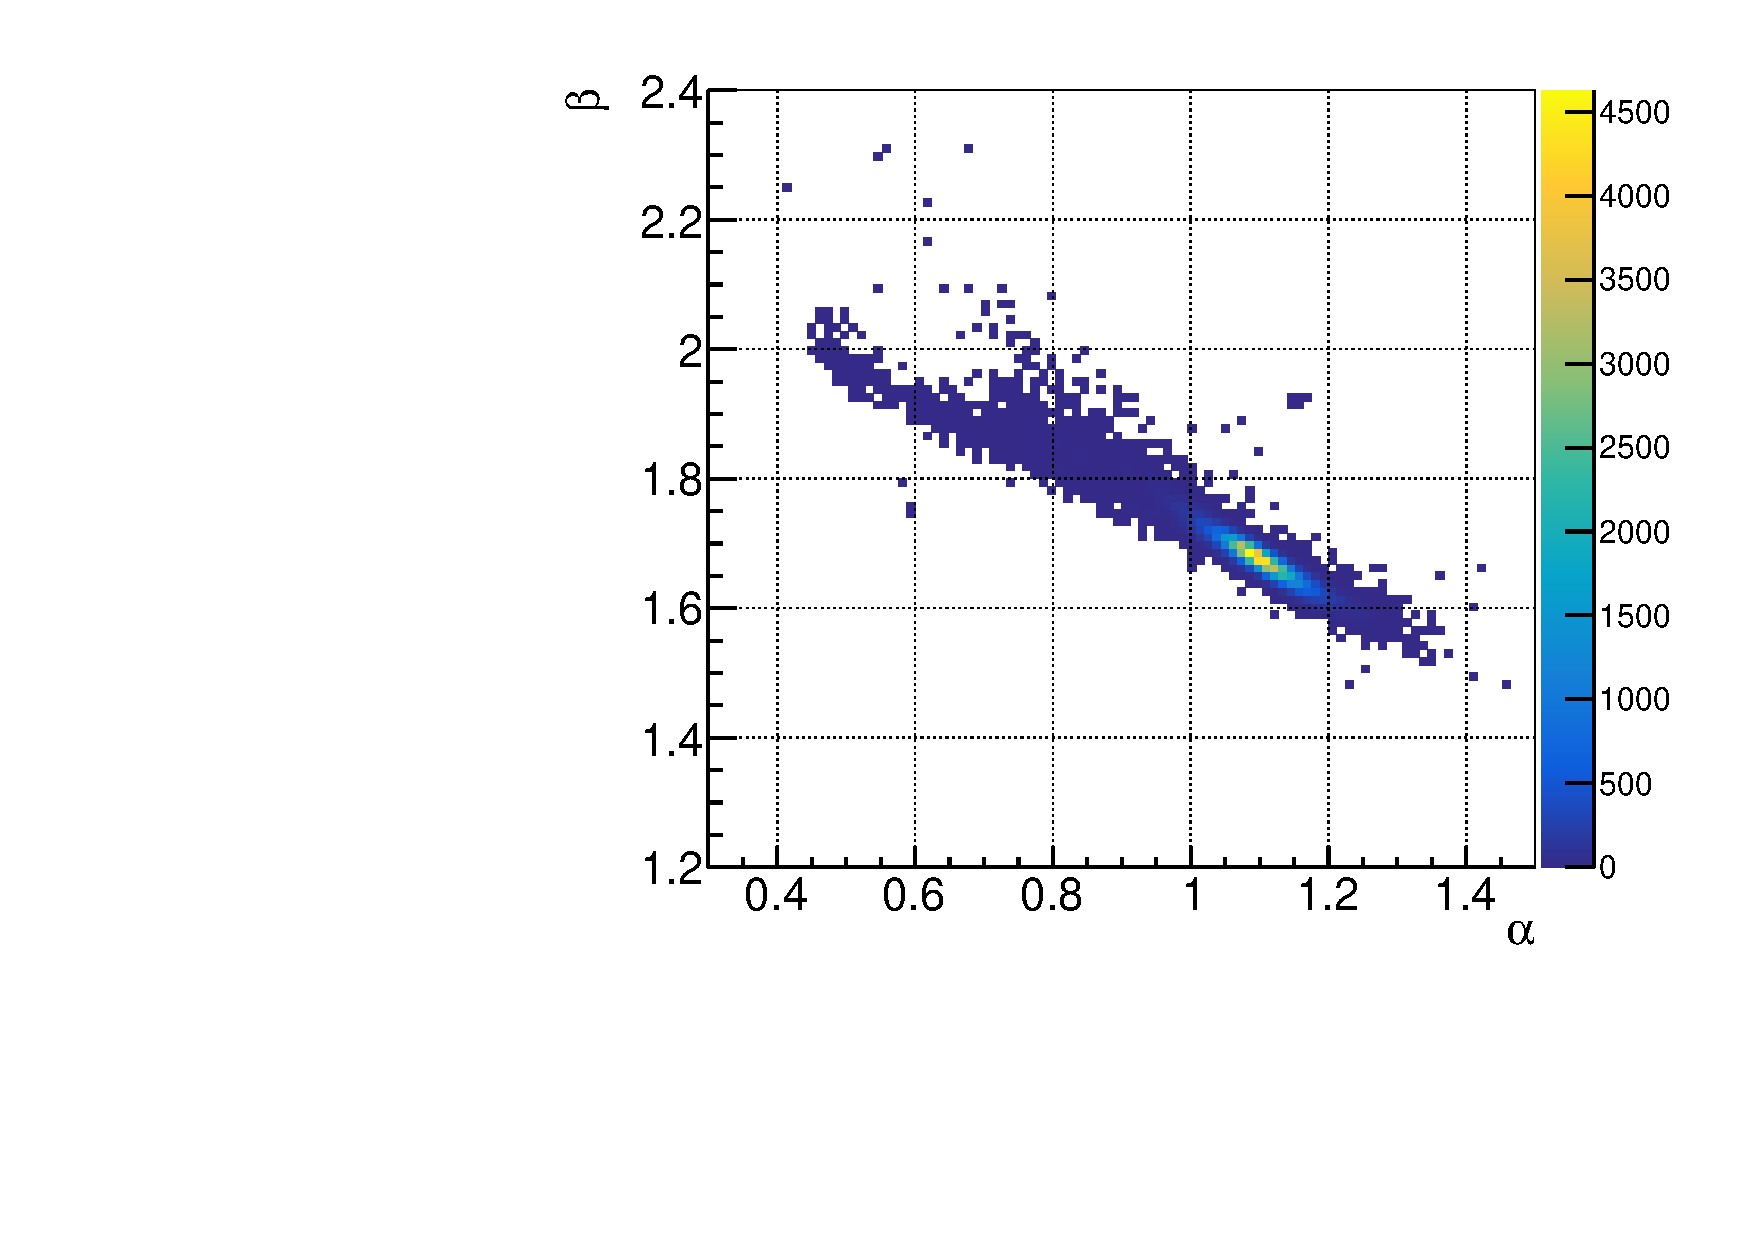
\includegraphics[]{Reconstruction/Figures/spikes/alphabeta_physical.pdf}
    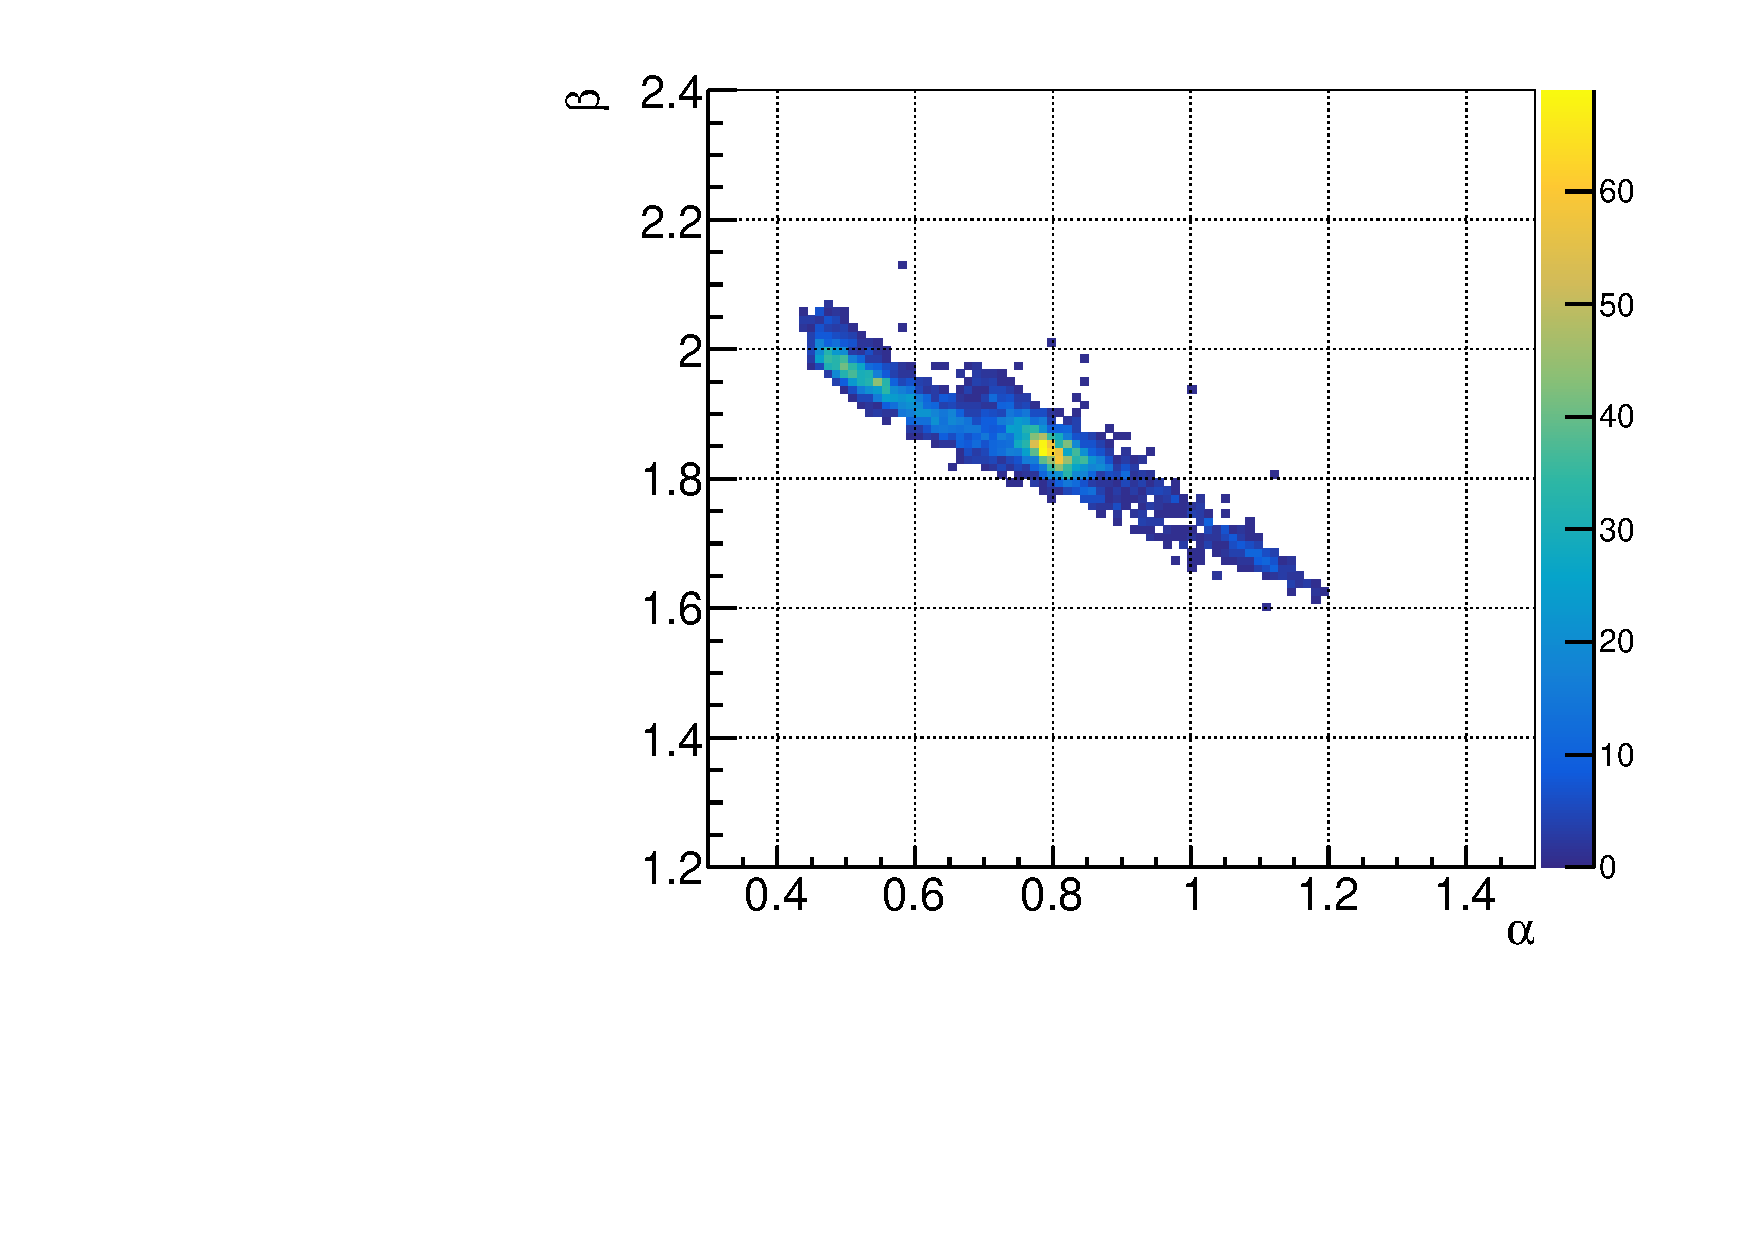
\includegraphics[]{Reconstruction/Figures/spikes/alphabeta_spike.pdf}
  }
  \caption{
    $\alpha$--$\beta$ distributions of the seed hits of physical wide clusters (left) and spike-like clusters (right).
  }
  \label{fig:spike_alphabeta}
\end{figure}

In the formula, parameters $A$ and $\tau$ correspond to the pulse amplitude and peak time, whereas $\alpha$ and $\beta$ control the shape of the pulse. 
Figure~\ref{fig:pulse_examples} illustrates various observed pulse shapes fit with the above formula with all parameters floating. 
A $\chi^{2}$ fit is employed using the average noise amplitude of each MGPA channel as the errors on the data points. 
The noise is measured in ECAL calibration cycles in the inter-fill period and is recorded in the conditions database.

\begin{figure}[htbp]
  \centering
  \resizebox{\textwidth}{!}{
    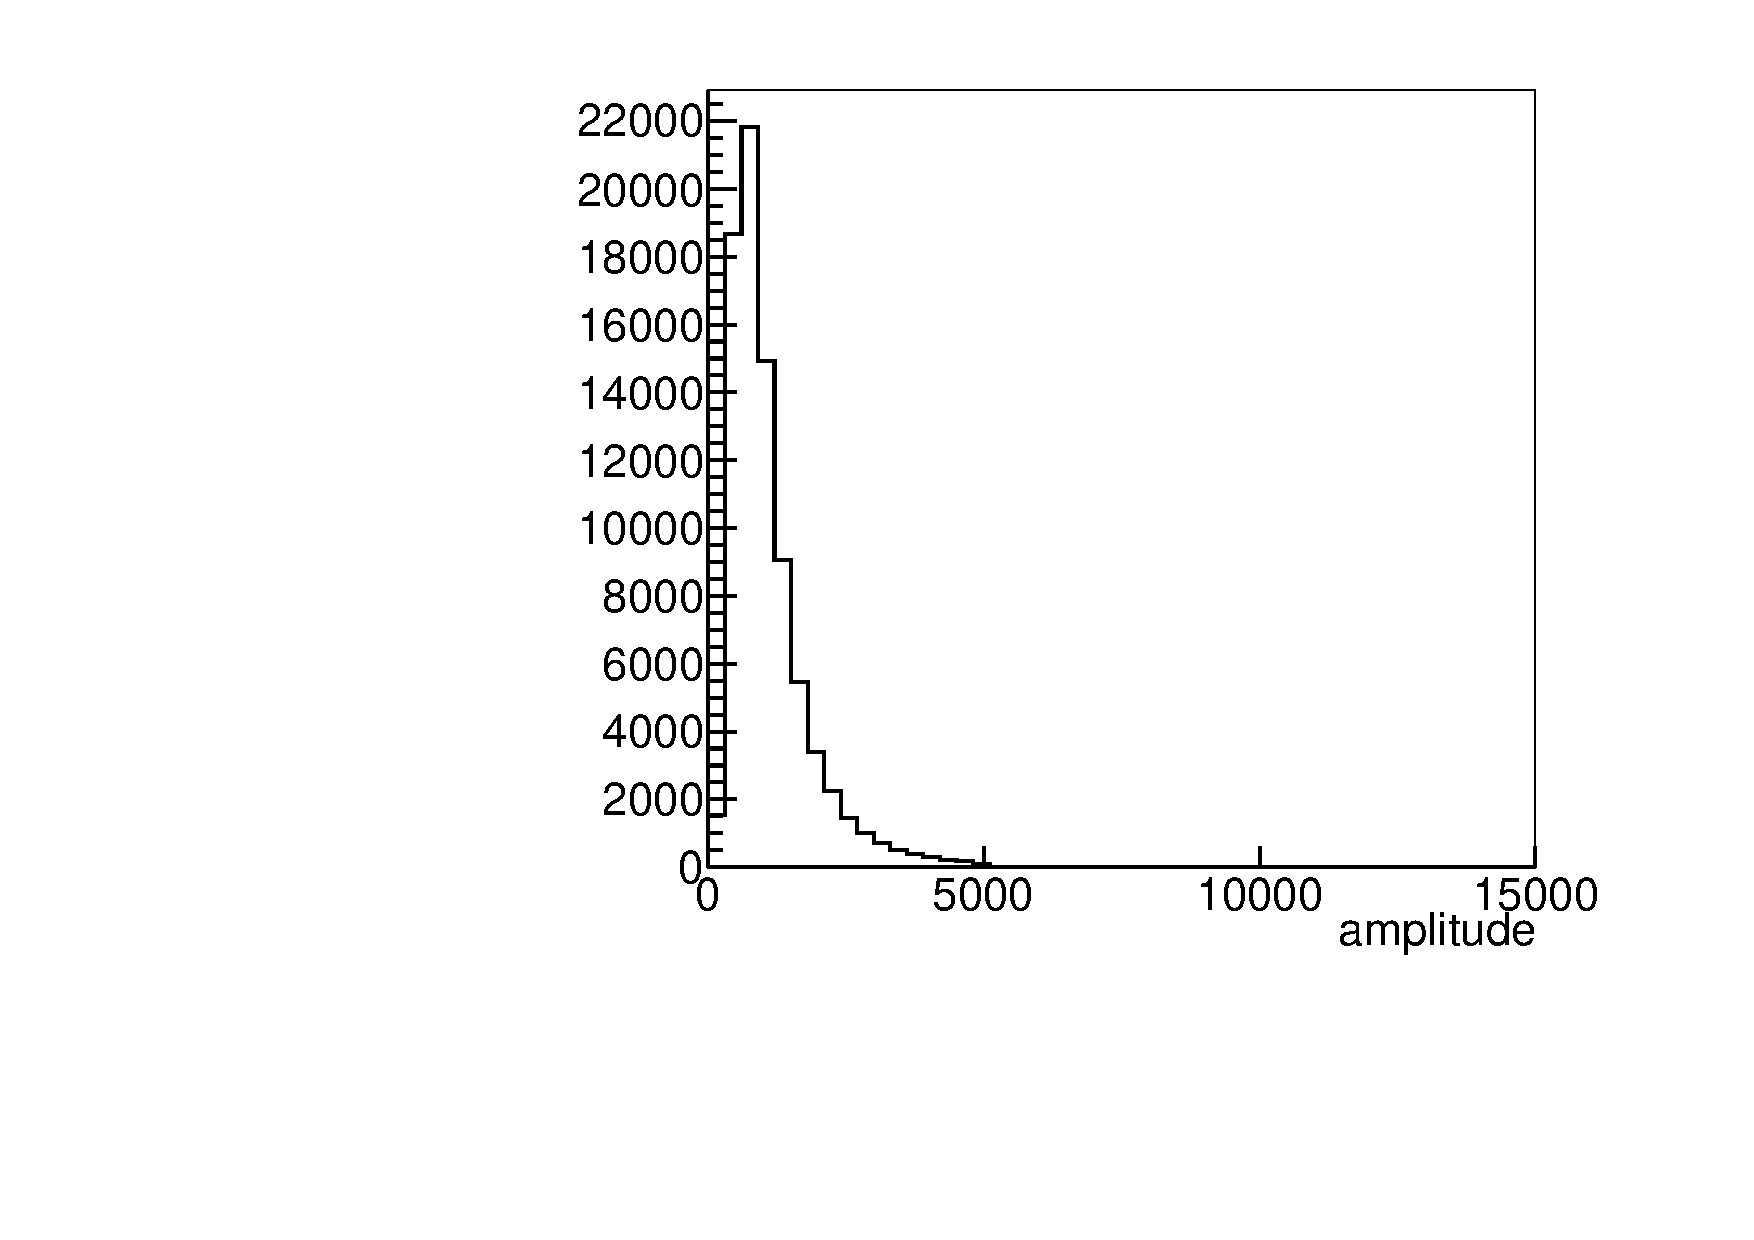
\includegraphics[]{Reconstruction/Figures/spikes/physical_amplitude.pdf}
    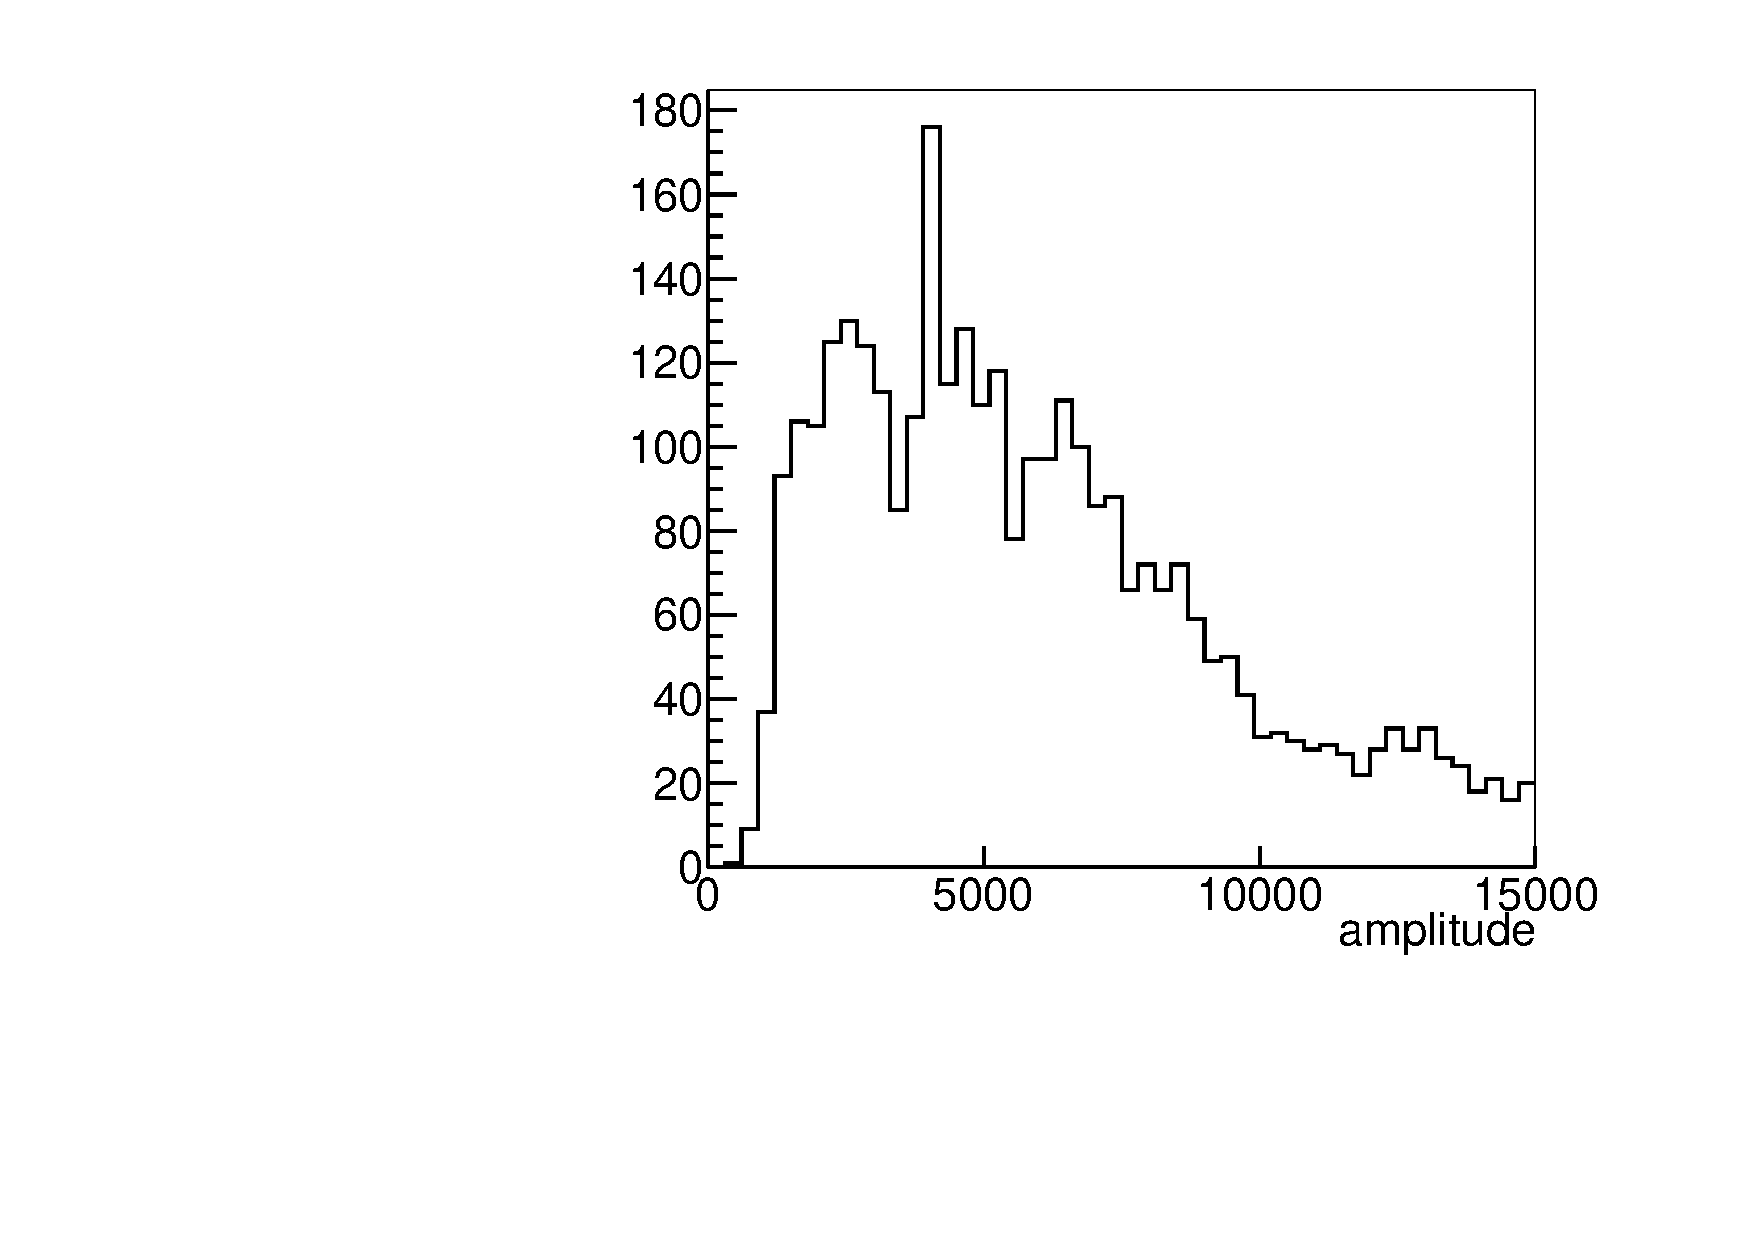
\includegraphics[]{Reconstruction/Figures/spikes/spike_amplitude.pdf}
    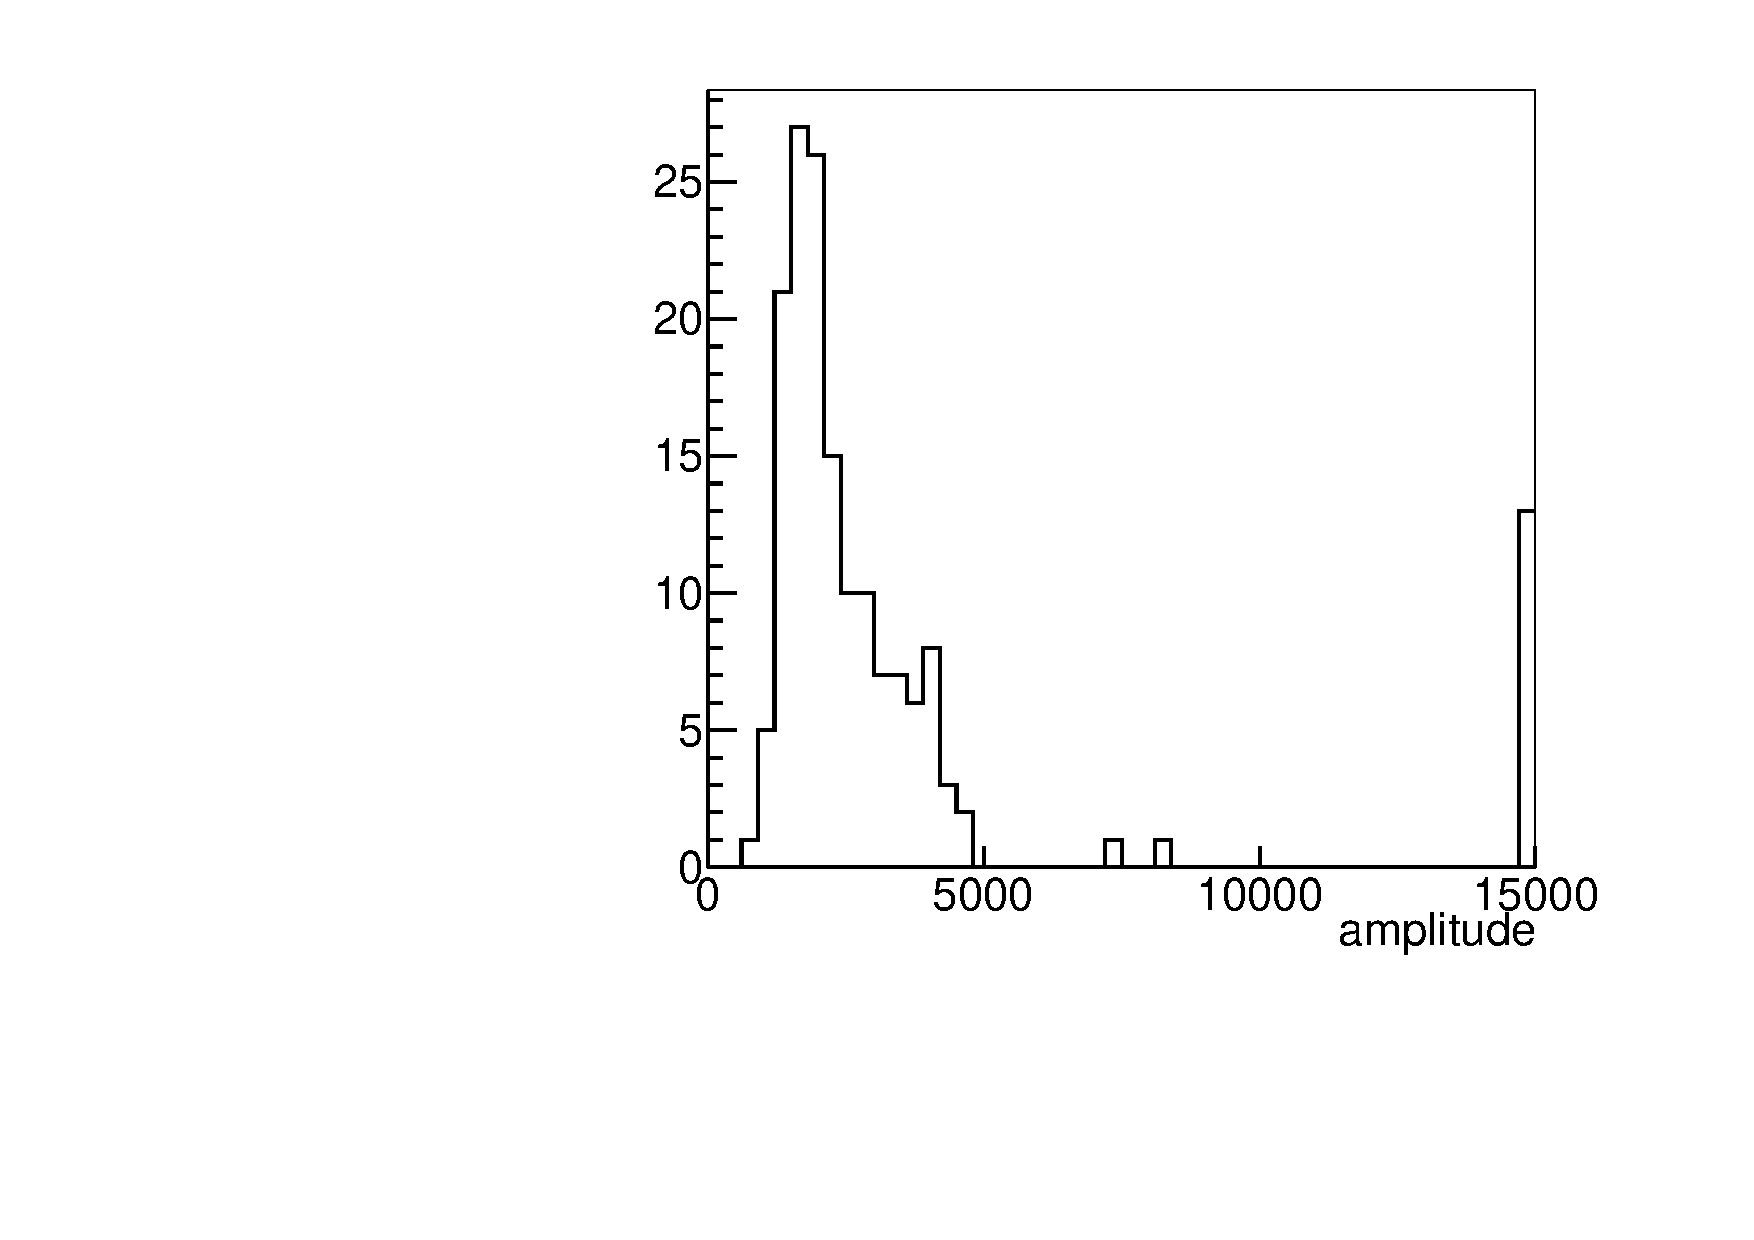
\includegraphics[]{Reconstruction/Figures/spikes/narrow_largealpha_amplitude.pdf}
    }
  \caption{
    Seed crystal pulse amplitude distributions of physical wide clusters (left), narrow clusters with $\alpha < 0.9$ (center), and narrow clusters with $\alpha > 0.9$ (right).
  }
  \label{fig:spike_amplitudes}
\end{figure}

In the $\alpha$--$\beta$ parameter space, seed rec hits of wide clusters concentrate around $(\alpha, \beta) \sim (1.1, 1.7)$, while spike-like hits populate the region $\alpha < 0.9$ as shown in Figure~\ref{fig:spike_alphabeta}.
In fact, the pulse amplitude distribution of narrow-cluster seeds with $\alpha > 0.9$ is unlike that of the narrow-cluster seeds with $\alpha < 0.9$, and resembles the amplitude distribution of wide-cluster seeds shown in Figure~\ref{fig:spike_amplitudes}.
This suggests that the population $\alpha > 0.9$ correspond to the clusters of physical, prompt photons.
It then follows that spike hits can be regarded to exclusively have
sharp pulse shapes. \PH{I am not sure you can definitively conlclude
  this, but all it does is just put a bound. So the method is fine,
  but I think you should be more exacting on the language.}

Given these observations, the time distribution of spike-like rec hits outside of the window $-15\ns < t < -10\ns$ (and the equivalent with one-bunch-crossing shift) is understood to be due to delayed interactions of neutral hadrons with the APDs, as documented also in Reference~\cite{CMS_AN_2010-357}. 
In other words, ECAL spike clusters which survive the time cleaning cut of the standard reconstruction are a part of a broad tail of a distribution, and there is no evidence of spike signals that specifically populate the ``in-time'' region $-3\ns < t < 3\ns$.

Having established that there is no special population of ECAL spikes in the in-time region, we can estimate the number $D$ of ECAL spike events present in the signal candidate sample to be
\begin{equation}
  D = C \times \frac{B}{A},
\end{equation}
where
\begin{itemize}
  \item A = Number of clusters with \sieie\ or \sipip\ less than 0.001 and seed time $-15\ns < t < -10\ns$, counted in the special-reconstruction sample,
  \item B = Number of clusters with both \sieie\ and \sipip\ greather than 0.001 and seed time $-15\ns < t < -10\ns$, counted in the special-reconstruction sample, 
  \item C = Number of clusters with \sieie\ or \sipip\ less than 0.001 but an in-time seed, counted in the standard-reconstruction sample passing all other signal event selection.
\end{itemize}

The special-reconstruction samples for A and B are from the SinglePhoton datasets, with only the timing cleaning removed from the offline reconstruction.
In this way, the selection bias over spikes from the L1T, HLT, and offline reconstruction is equally applied to samples A, B, and C. Plugging in the observed numbers, we have
\begin{align*}
  A & = 4969 \\
  B & = 1180 \\
  C & = 54 \\
  \therefore D & = 12.8 \pm 1.8 \text{(stat.)}
\end{align*}

There are, however, at least two reasons to believe that this method overestimates the number of spike events in the signal region. 
One is that the population C contains some physical, prompt photon clusters that just happen to be narrow, as observed in Fig.~\ref{fig:sieie_mc}. 
Another reason is that there is likely a correlation between the cluster width and the seed time such that the ratio of true D to C is smaller than $B/A$.
This statement is based on the standard hypothesis that the wide-cluster spike is an ECAL spike embedded in a physical EM shower cluster. 
Under this model, spikes in wide clusters are mainly caused by prompt neutral hadrons in a jet, which implies that they strongly prefer seed time $-15\ns < t < -10\ns$. 
Given that this is a minor background with a relatively large uncertainty, as described below, we will still use this estimate as the nominal value of predicted spike contribution in the signal region.

The uncertainty in the estimate of D is evaluated by two modifications to A, B, and C.
First, the three values are recomputed with using $\sieie < 0.001$ as the only definition of narrow cluster. 
This results in a minor change of the value of D of $12.1 \pm 1.7$. Next, A and B are computed using a lower-\pt SinglePhoton sample, requiring triggers \texttt{Photon135\_PFMET100} or \texttt{Photon120\_R9Id90\_HE10\_IsoM} to have fired, instead of the signal trigger. 
The second modification gives $D=9.1 \pm 1.3$. 
We then take twice the discrepancy between the nominal D and the D value from the second modification to obtain a 33\% systematic uncertainty on the spike background estimate.
\PH{Are you not using hte signal region for the spike
  estimate. Perhaps you can add some text to justify this is ok. }
